\section{VDMS Design \& Implementation}
\label{arch}

In this section, we describe VDMS design principles and implementation,
which was briefly introduced in previous work \cite{vdms-nips}.
Figure \ref{fig:arch} depicts the high-level architecture of VDMS.
VDMS implements a client-server architecture that handles client
requests concurrently, and coordinates query execution across
the metadata and visual data components in order to return a unified response.
Users interact with both metadata and visual data
(i.e., images, videos, feature vectors) using a unified API,
in a transactional manner.

The metadata component is the \textit{Persistent Memory Graph
Database} (PMGD) and the (visual) data component is our Visual Compute Module.
The Visual Compute Module enables machine-friendly enhancements to
visual data, exposing high-level abstractions to the \textit{Request Server}
for dealing with a variety of images and video formats (through OpenCV and ffmpeg),
and different methods for indexing for feature vectors
(including Facebook's Faiss \cite{faiss}, TileDB \cite{TileDB}).
Finally, a main component of VDMS is in charge of implementing the API and orchestrating between the PMGD and the Visual Compute Module
to serve client's requests. This component is the \textit{Request Server}.

VDMS and its components are fully available as open source projects
\footnote{https://github.com/IntelLabs/\{vdms, pmgd\}}.
We briefly describe each of the main components as follows:

\begin{figure}
\centering
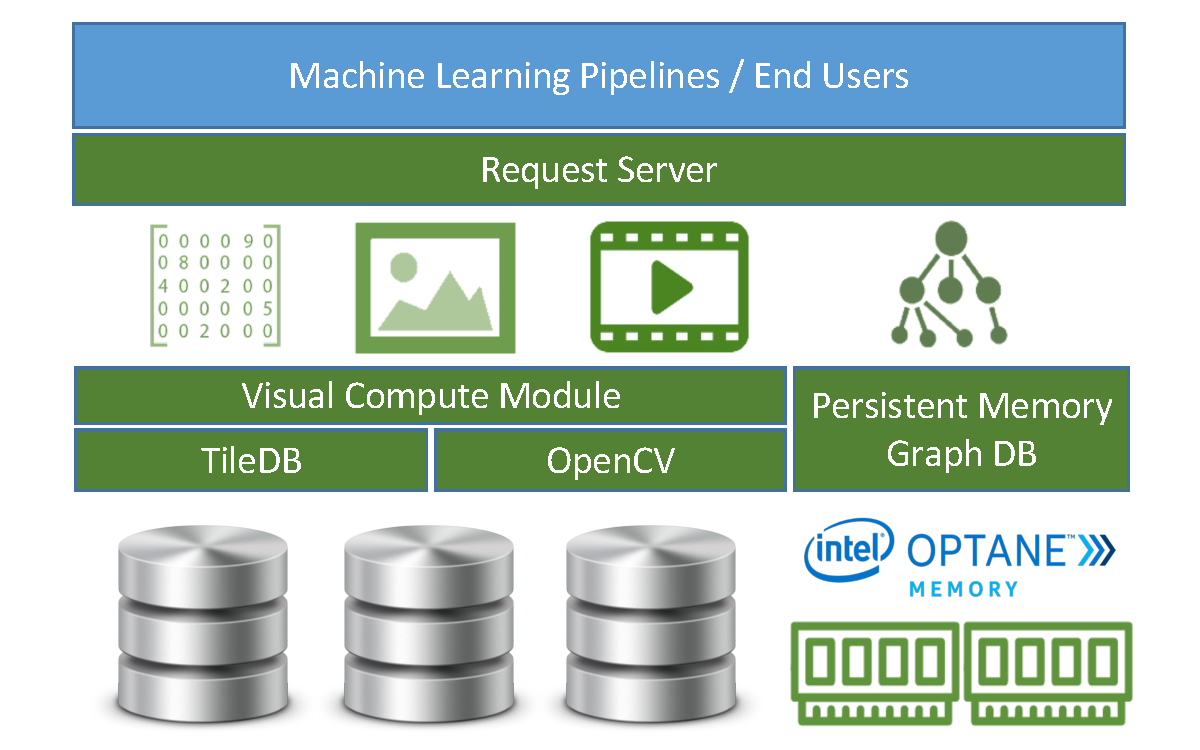
\includegraphics[width=1\columnwidth]{figures/vdms_arch.pdf}
\caption{VDMS Architecture}
\label{fig:arch}
\end{figure}

\subsection{Persistent Memory Graph Database}

We use the Persistent Memory Graph Database (PMGD) to provide an efficient storage
solution addressing the increasing popularity of connected data and
applications that benefit from graph-like processing.
PMGD implements an in-persistent-memory graph database, PMGD, optimized
to run on a platform equipped with persistent memory.
PMGD provides a property graph model of data storage with the traditional
atomicity, consistency, isolation, and durability
(ACID) properties expected from databases.
Graph represents an easier abstraction to model complex problems \cite{tao}.
Moreover, the graph model makes it very suitable for the data and
access patterns shown by visual metadata, which can be easily mapped
into application-level abstractions by developers.
For instance, abstractions like \textit{BoundingBoxes} associated to
images or videos can be easily represented using nodes and edges.
With its natural ability to extend the schema very
easily (due to the use of a property graph model),
we can support new developments in machine learning that can lead to
enhancements to existing metadata over time.
These are the reasons the team chose a graph database over a
relational database as the metadata management for the implementation of VDMS.
PMGD is designed and optimized for persistent memory technologies
like Intel Optane~\cite{IntelXPoint15}, which
promise storage providing nearly the speed of DRAM and the
durability of block-oriented storage.

\subsection{Visual Compute Module}

The Visual Compute Module was designed and implemented to provide
an internal abstraction layer for interacting with visual data.
It enables simple visual data handling and processing (i.e., basic building block
operations like crop, resize, etc).
For traditional formats (jpg, png, tiff, mp4, etc.),
the interface is an abstraction layer over OpenCV.
However, it also provides a way to use novel formats that are
better suited for visual analytics: a novel, array-based lossless image format.
This format is built on the array data manager TileDB~\cite{TileDB} and
is well suited for images that are used in visual analytics.

VDMS provides full support for video storage and operations,
in a similar way it does for images.
This includes support for encoding, decoding, and transcoding of
\textit{mp4}, \textit{avi}, and \textit{mov} containers,
as well as support for \textit{xvid}, \textit{H.263} and \textit{H.264} encoders.
This is supported through the use of either OpenCV~\cite{opencv}
or \textit{libffmpeg}\cite{ffmpeg}, or both.
All operations supported for images in VDMS are also supported at the
video and frame level of the API.
On top of that, there are a number of video-specific operations that
are supported, such as the interval operations,
enabling users to retrieve clips at different
frames-per-second (FPS) versions of the video.

Another key differentiating factor of VDMS is that it allows the creation of
indexes for high-dimensional feature vectors and the insertion of
these feature vectors associated with entities, images, and/or videos.
Feature vectors are intermediate results of various machine
learning or computer vision algorithms when run on visual data.
Feature vectors are also known as \textit{descriptors}
or \textit{visual descriptors}.
We use these terms interchangeably.
These descriptors can be classified, labeled, and used to build search indexes.
Feature Vectors support is provided through our implementation based
on high-dimensional sparse arrays, also using TileDB.
In addition, the Visual Compute Library provides a wrapper
for another high-dimensional index implementation,
Facebook's Faiss~\cite{faiss}.

\subsection{Request Server}

Developers and users of machine learning frameworks and data science
applications favor simpler interfaces to access and process data.
They cannot be expected to deal with two different ways of interacting
with information (metadata and visual data) instead of focusing on the
algorithmic parts of their pipelines.
VDMS takes care of coordinating client requests across the metadata and the
visual data, and managing multiple clients through the \textit{Request Server}.
The \textit{Request Server} is a key component of the system,
as it implements VDMS' API and coordinates request and responses from
the PMGD and Visual Compute Module subsystems.
It decomposes the user queries into
metadata and visual data requests, invokes the relevant calls behind the scene,
and returns a coherent and unified response that is easy for the user to parse
and interpret.

\subsection{VDMS API}

One of the most important differentiating factor of VDMS is its interface.
VDMS is unique in recognizing visual entities (i.e., images, videos, etc)
as first class citizens. Thus, VDMS provides an API that revolves
around visual data operations and retrieval.
VDMS API is easy to use and explicitly pre-defines certain
primitives associated with metadata, images, videos, and feature vectors.
Authors have paid particular attention to hide the complexities of our internal
implementation and up-level the API to a JSON-based API,
which is very popular across various application domains.
By defining a new JSON-based API, there is a trade-off between expressiveness
(compared to well-established query languages like SPARQL, Gremlim, or even SQL)
and the ability to natively support visual data operations.
However, we believe it is possible for our API to achieve similar levels of
expressiveness compared to more mature query languages over time.

Listing~\ref{findimagegeo} shows a sample query.
In this particular example, the transaction retrieves
all the images of \textit{alligators}
with probability higher than 0.66,
filter by latitude and longitude within 1 degree,
apply a resize operation to make the images 224x224,
rotate the images 45.34 degrees,
and return the images as "png" files.
It is important to note how the API natively supports basic building
blocks of visual data processing, like resize, rotation, or transcoding
(changing output formats and encodings).
The API allows interaction with metadata, images, videos,
and feature vectors in a similar fashion, and it is fully
documented on the project's Github
wiki~\footnote{https://github.com/IntelLabs/vdms/wiki/API-Description}.

\begin{listing}[ht!]
\begin{minted}[frame=single,
              framesep=3mm,
              linenos=true,
              xleftmargin=21pt,
              tabsize=4]{js}
"FindEntity"{
    "class": "autotag",
    "constraints": {
        "name": ["==", "alligator"]
    }
    "_ref" : 1
},
"FindImage":{
    "format": "png",
    "link": {
        "ref":1,
        "constraints": {
            "prob": [">=", 0.66]
        }
    },
    "constraints": {
        "latitude": [">=", 36.23433,
                     "<=", 38.23433]
        "longitude":[">=", -114.80666,
                     "<=", -116.80666]
    },
    "operations": [{
        "type": "resize",
        "height": 224,
        "width":  224,
    }, {
        "type": "rotate",
        "angle": 45.34
    }]
}

\end{minted}
\caption{Sample Query for Image Retrieval -
The query expresses the following:
Find all the images connected to the autotag \textit{alligator}
with probability higher than 0.66,
filter the images by latitude and longitude within 1 degree,
apply a resize operation to make the images 224x224,
rotate the image 45.34 degrees,
and return the images as "png" files.}
\label{findimagegeo}
\end{listing}

\subsection{Client Library}

The client library implements TCP/IP based connectors to the VDMS Server,
similar to most database\cite{memsql, mysql}.
Users can connect to VDMS and implement queries using VDMS' API
by defining JSON commands conforming to the query protocol we have defined.
The client library provides a simple method that
accepts a JSON string and an array or vector of blobs.
Internally, the library wraps the query string and blob using
Google Protobufs \cite{protobufs} and sends it to the VDMS server.
It also receives a similarly formed response from VDMS
and returns it to the client.
The responses require JSON parsing on the client
side for the metadata string that indicates how to interpret the blobs field.
Currently, client libraries are implemented for Python and C++ client.
The client libraries are lightweight, as they simply implement the communication
protocol between the client and the server.
This makes it easier for developers to implement similar client libraries using
any other programming language of their choice.
